\chapter{File System}
Il file system è una delle parti del sistema operativo più importanti per l'utente perché si occupa della gestione dei file. I file, a loro volta, sono l'elemento principale della maggior parte delle applicazioni perché hanno un'esistenza a lungo termine (in genere "sopravviviono" ai processi), possono essere condivisi con altri processi e sono strutturati in directory gerarchiche. Le operazioni tipiche sui file sono: creazione, cancellazione, apertura, scrittura e chiusura. I file sono gestiti da un insieme di programmi e librerie di utilità che costituiscono il \textit{File Management System}, e vengono eseguiti come processi privilegiati. I File Management Systems forniscono servizi agli utenti e alle applicazioni per l'uso di file e definiscono anche il modo in cui i file sono usati, in questo sollevano i programmatori dal dover scrivere codice per gestire i file.

L'organizzazione tipica richiede un Directory Management che si occupa di tutte le operazioni utente che hanno a che fare con i file; un File System che gestisce la struttura logica e le operazioni (apri, chiudi, leggi, scrivi...); l'organizzazione fisica che identifica i file con indirizzi fisici su disco.

\section{Directory}
Una directory è un file "speciale" che permette di mappare i nomi dei file alle loro informazioni. Le operazioni consentite su una directory sono: ricerca, creazione file, cancellazione file, lista del contenuto, modifica. A parte le informazioni dei file (nome, tipo e organizzazione del file), una directory deve contenere: il volume, indica il dispositivo su cui il file è memorizzato; l'indirizzo di partenza, ad es.: da quale settore o traccia di disco; la dimensione attuale, in byte, word o blocchi; la dimensione allocata, dimensione massima del file; il proprietario, può concedere/negare i permessi ad altri utenti, e può anche cambiare tali impostazioni; le informazioni sull'accesso, potrebbe contenere username e password per ogni utente autorizzato; le azioni permesse, per controllare lettura, scrittura, esecuzione, spedizione tramite rete; i time stamp di creazioni, accessi, identità e backup. 

Il metodo usato per memorizzare queste informazioni è con uno schema gerarchico ad albero, dove c'è una \textit{directory master} che contiene le \textit{directory utente} e, ogni directory utente può contenere alte directory oppure altri file (vedi Figura \ref{fig:esempio-albero-file}). La struttura ad albero permette agli utenti di trovare un file seguendo un percorso nell'albero (\textit{directory path}) e file con nomi duplicati sono possibili purché con path diversi.

\begin{figure}[h]
    \centering
    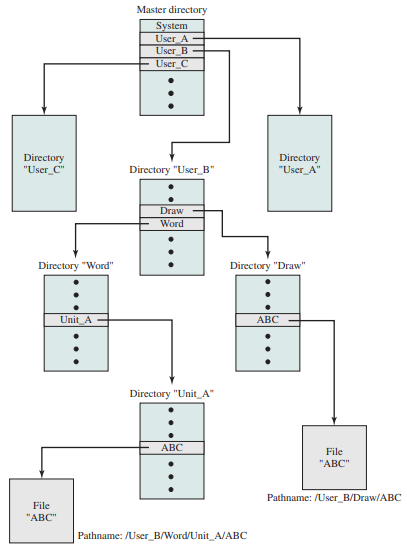
\includegraphics[width=0.4\linewidth]{images/esempio-albero-file.PNG}
    \caption{Esempio di struttura ad albero}
    \label{fig:esempio-albero-file}
\end{figure}

Dover dare ogni volta il path completo prima del nome del file può essere lungo e noioso, quindi solitamente, gli utenti o i processi interattivi hanno associata una \textit{directory di lavoro} o corrente dove tutti i nomi di file sono dati relativamente a questa directory.

\section{Gestione della memoria secondaria}
Il sistema operativo è responsabile dell'assegnamento di blocchi a file e per tanto occorre allocare e mantenere traccia dello spazio per i file e occorre tener traccia dello spazio allocabile. I file vengono allocati in porzioni o blocchi, ovvero in sequenze contigue di settori di disco. 

\subsection*{Allocazione dei file}
L'allocazione dinamica è quasi sempre preferita, perché altrimenti con la preallocazione viene riservato lo spazio massimo stimato durante la sua creazione del file con risultante spreco di spazio su disco. 

Per l'allocazione delle porzioni ci sono due possibilità: o si alloca una porzione larga a sufficienza per l'intero file, è un approccio efficiente per il processo che vuole creare il file, oppure si alloca un blocco alla volta in una sequenza di settori contigui, è efficiente per il sistema operativo che deve gestire tanti file. Si cerca un punto d'incontro tra efficienza del singolo file ed efficienza del sistema con porzioni grandi di dimensione variabile oppure con porzioni fisse piccole.

Per allocare spazio per i file si usano principalmente tre metodi: contiguo, concatenato, indicizzato. Vediamoli nel dettaglio:
\begin{itemize}
    \item Con l'\textit{allocazione contigua} viene allocato un insieme di blocchi per il file quando quest'ultimo viene creato, quindi è necessaria la preallocazione. Nella tabella di allocazione c'è una sola entry contenente il blocco di partenza e la lunghezza del file e c'è bisogno di compattare i settori quando i file vengono eliminati (frammentazione esterna).
    
    \item Con l'\textit{allocazione concatenata} viene allocato un blocco alla volta e ogni blocco contiene una parte relativa ai dati del file e una per il puntatore al blocco successivo. E' necessaria una sola entry nella tabella di allocazione dei file che contiene il blocco di partenza e la lunghezza del file. Questo metodo risulta utile quando bisogna accedere sequenzialmente ai file e utilizzando il consolidamento si inseriscono i file contigui in modo da migliorare anche l'accesso non sequenziale.

    \item L'\textit{allocazione indicizzata} è una via di mezzo tra i due approcci precedenti dove i blocchi possono contenere dati oppure indici. Infatti, nella tabella di allocazione dei file, si ha una sola entry con l'indirizzo di un blocco, questo blocco contiene degli indici per ogni porzione allocata al file. I blocchi possono avere lunghezza fissa o variabile e nel secondo caso oltre agli indici deve essere specificata anche la lunghezza di ogni blocco.
\end{itemize}


\begin{Example}{Allocazione}{}
    \textit{Supponiamo di avere 35 settori e analizziamo gli approcci di allocazione di spazio per i file.}
    
    Con l'allocazione contigua per ogni file viene deciso il blocco di partenza e la sua lunghezza tenendo conto della dimensione massima stimata:
    
    \begin{minipage}{\textwidth}
        \centering
        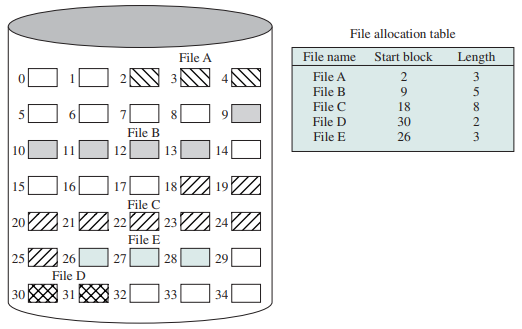
\includegraphics[width=0.49\linewidth]{images/allocazione-contigua.PNG}
        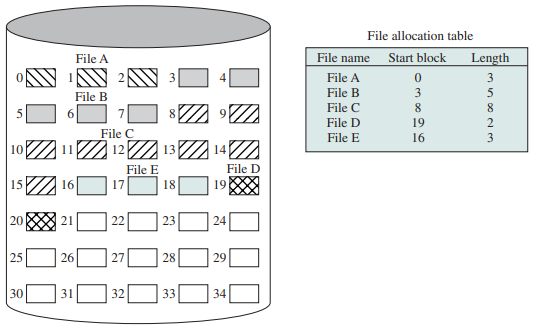
\includegraphics[width=0.49\linewidth]{images/allocazione-contigua2.PNG}
        \captionof{figure}{Allocazione contigua e compattazione}
    \end{minipage}\\

    Con l'allocazione concatenata nella tabella di allocazione dei file troviamo solo il file iniziale con la sua lunghezza:
    
    \begin{minipage}{\textwidth}
        \centering
        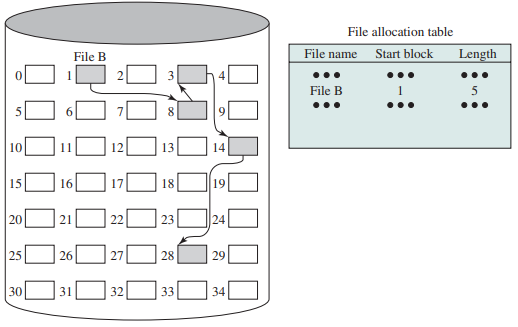
\includegraphics[width=0.49\linewidth]{images/allocazione-concatenata.PNG}
        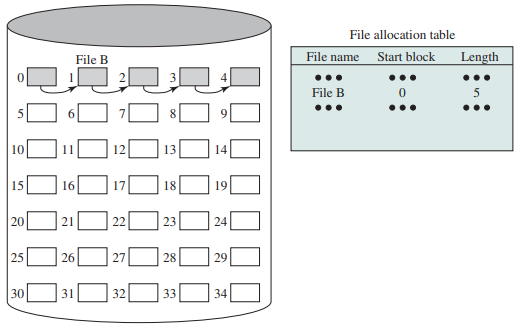
\includegraphics[width=0.49\linewidth]{images/allocazione-concatenata2.PNG}
        \captionof{figure}{Allocazione concatenata e consolidamento}
    \end{minipage}\\

    Con l'allocazione indicizzata l'indirizzo dell'unica entry della tabella contiene gli indici di ogni porzione allocata al file:
    
    \begin{minipage}{\textwidth}
        \centering
        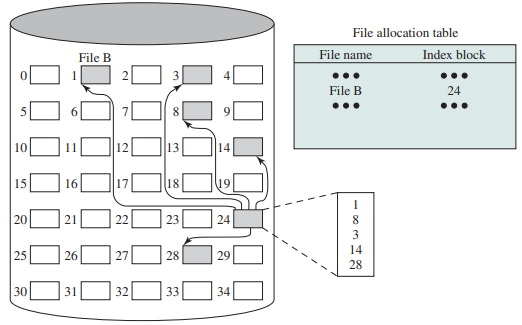
\includegraphics[width=0.49\linewidth]{images/allocazione-indicizzata.PNG}
        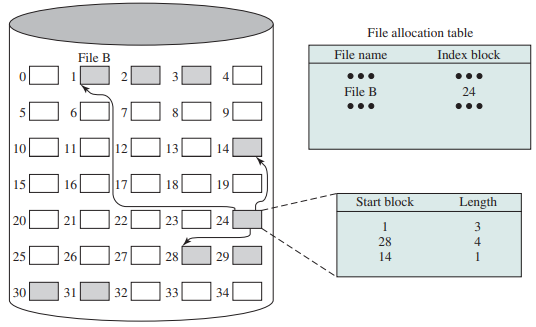
\includegraphics[width=0.49\linewidth]{images/allocazione-indicizzata2.PNG}
        \captionof{figure}{Allocazione indicizzata con porzioni fisse e variabili}
    \end{minipage}
\end{Example}

\subsection*{Gestione dello spazio libero}
La gestione dello spazio libero è altrettanto importante di quello occupato. Per gestire lo spazio libero serve una tabella di allocazione di disco, oltre che a quella di allocazione per i file e ogni volta che si alloca o si cancella un file, lo spazio libero va aggiornato. Per fare ciò ci sono vari approcci:
\begin{itemize}
    \item La \textit{tabella di bit} è un vettore con un bit per ogni blocco su disco (0 libero, 1 occupato). In questo modo si minimizza lo spazio richiesto alla tabella di allocazione del disco ma se il disco è quasi pieno, la ricerca di uno spazio libero può richiedere molto tempo.

    \item Le porzioni libere possono essere \textit{concatenate} tra loro usando, per ogni blocco libero, un puntatore ed un intero per la dimensione, il tutto senza overhead di spazio. Però, se c'è molta frammentazione, la lista diventa inevitabilmente lunga e se bisogna allocare molti file si devono leggere altrettanti blocchi per sapere qual'è il prossimo libero.

    \item Si può trattare lo spazio libero come un unico file, ovvero con una entry e con un \textit{indice} che gestisce le porzioni come se fossero di lunghezza variabile.

    \item Con la \textit{lista dei blocchi liberi} ad ogni blocco libero viene assegnato un numero sequenziale e la lista di questi numeri viene memorizzata in una parte dedicata del disco.
\end{itemize}

Un \textit{volume} è un insieme di settori in memoria secondaria, che possono essere usati dal sistema operativo o dalle applicazioni.

I \textit{dati} rappresentano il contenuto dei file, mentre i \textit{metadati} sono tutte le altre informazioni (lista di blocchi liberi, data dell'ultima modifica...). I metadati devono essere su disco, perché devono essere persistenti, ma mantenerli sempre costanti è inefficiente per questo, tramite il \textit{journaling}, anziché scrivere le informazioni nelle opportune porzioni di disco, le si scrive in una zona di disco dedicata (\textit{log}).

\section{Gestione dei file in UNIX}
In UNIX ci sono sei tipi di file: normale, directory, speciale (mappano su nomi di file i dispositivi di I/O), named pipe (per far comunicare processi tra loro), hard link (collegamenti, nome di file alternativo), link simbolico (il suo contenuto è il nome del file cui si riferisce).

\subsection*{Inode}
Un \textit{inode} (index node) è una struttura dati che contiene le informazioni essenziali per un dato file e ogni inode è identificato con un numero per garantire un accesso più semplificato. Dal sistema operativo viene mantenuta una tabella di tutti gli inode corrispondenti a file aperti in memoria principale, e tutti gli altri i-node sono in una zona di disco dedicata (i-list). Ogni inode contiene le seguenti informazioni: tipo e modo di accesso del file; identificatore dell'utente proprietario e del gruppo cui tale utente appartiene; tempo di creazione e di ultimo accesso (lettura o scrittura); flag utente e flag per il kernel; numero sequenziale di generazione del file; dimensione delle informazioni aggiuntive; altri attributi (controllo di accesso e altro); dimensione; numero di blocchi o numero di file (per le directory); dimensione dei blocchi; sequenze di puntatori a blocchi.

\begin{figure}[h]
    \centering
    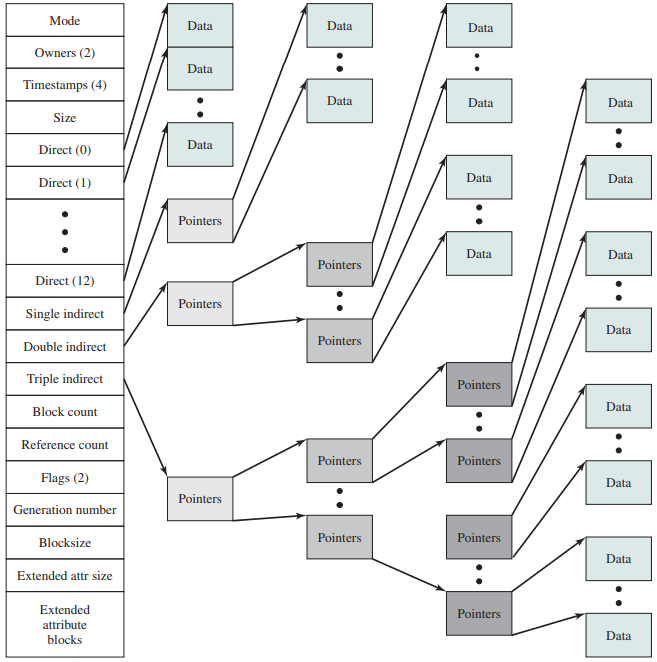
\includegraphics[width=0.5\linewidth]{images/inode.PNG}
    \caption{inode}
    \label{fig:inode}
\end{figure}

\subsection*{Allocazione, directory e accesso ai file}
L'\textit{allocazione} in UNIX è dinamica a blocchi e l'indicizzazione tiene traccia dei blocchi dei file.

Le \textit{directory} sono file che contengono una lista di coppie formata da un puntatore all'inode e il nome del file. Alcuni di questi file potrebbero essere a loro volta directory, quindi si forma una struttura gerarchica dove ogni directory può essere modificata solo dal sistema operativo, ma letta da ogni utente.

\begin{figure}[h]
    \centering
    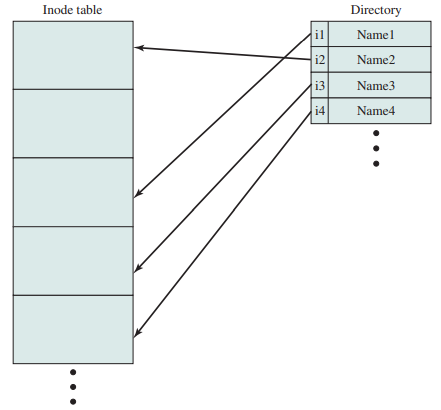
\includegraphics[width=0.4\linewidth]{images/directory-inode.PNG}
    \caption{Directory e inode}
    \label{fig:directory-inode}
\end{figure}

Per l'\textit{accesso ai file} ci sono tre terne di permessi: lettura, scrittura e esecuzione che a loro volta vengono gestiti nella terna di proprietario, il suo gruppo e tutti gli altri. Quindi, per ogni file, si gestiscono opportunamente i permessi di lettura, scrittura ed esecuzione per \verb|user|, \verb|group| e \verb|other|.

\begin{figure}[h]
    \centering
    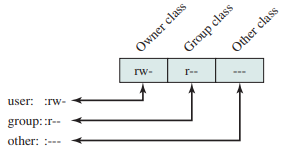
\includegraphics[width=0.4\linewidth]{images/accesso-file.PNG}
    \caption{Accesso ai file}
    \label{fig:accesso-file}
\end{figure}

\section{Gestione dei file su Windows}
In Windows ci sono due file system principali: \textit{FAT} (File Allocation Table - vecchio file system) con allocazione concatenata e blocchi di dimensione fissa; \textit{NTFS} (New Technology File System - nuovo file system) con allocazione con bitmap e blocchi di dimensione fissa.

\subsection*{File Allocation Table}
La\textit{ File Allocation Table}, è una tabella ordinata di puntatori, ancora in uso per le chiavette USB, e usa un puntatore (riga nella tabella) per ogni cluster del disco. Ogni cluster ha dimensione variabile tra 2 e 32 KB, ed
è costituito da settori di disco contigui, di conseguenza, la tabella cresce con la grandezza della partizione. La parte della FAT relativa ai file aperti deve essere sempre mantenuta interamente in memoria principale per consentire di identificare i blocchi di un file e accedervi sequenzialmente seguendo i collegamenti nella FAT.

Ogni FAT contiene delle regioni di informazioni (vedi Figura \ref{fig:fat-regioni}): \textit{Regione Boot Sector} contiene informazioni necessarie per l'accesso al volume; \textit{Regione FAT} contiene due copie della file allocation table e mappa il contenuto della regione dati, indicando a quali directory/file i diversi cluster appartengono; \textit{Regione Root Directory} è una directory table che contiene tutti i file entry per la directory root del sistema; \textit{Regione Dati} è la regione del volume in cui sono effettivamente contenuti i dati dei file e directory.

\begin{figure}[h]
    \centering
    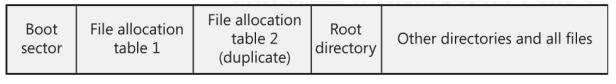
\includegraphics[width=0.5\linewidth]{images/fat-regioni.PNG}
    \caption{Regioni della FAT}
    \label{fig:fat-regioni}
\end{figure}

Data la tabella FAT di puntatori, il puntatore i-esimo, se è 0, indica che l'i-esimo cluster del disco è libero; se è tutti 1 (valore speciale), indica che ci troviamo sull'ultimo blocco del file; se non è 0 e non è un valore speciale, indica il cluster dove trovare il prossimo pezzo del file, oltre che la prossima entry della FAT per questo file (vedi Figura \ref{fig:fat}).

\begin{figure}[h]
    \centering
    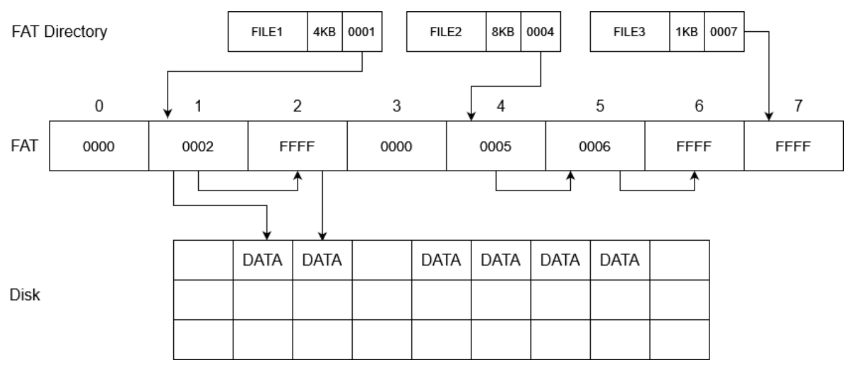
\includegraphics[width=0.7\linewidth]{images/fat.PNG}
    \caption{Funzionamento della FAT}
    \label{fig:fat}
\end{figure}

\subsection*{New Technology File System}
Nell'NTFS i file sono definiti da un insieme di attributi rappresentati come un byte stream. Anche in questo file system ci sono diverse regioni: \textit{Regione Boot Sector} è basata sull'equivalente FAT; \textit{Master File Table} è la principale struttura dati del file system implementata come un file con una sequenza lineare di record, dove ogni record descrive un file identificato da un puntatore. 

NTFS cerca sempre di assegnare ad un file sequenze contigue di blocchi e per ogni file, esiste un record base nell'MFT. NTFS usa una tecnica simle agli i-node UNIX/Linux: il record base è un puntatore a n record secondari, eventuale spazio rimanente nel record base contiene le prime sequenze del file; se i record estesi non rientrano in MFT per mancaza di spazio, vengono quindi salvati in un file dedicato, con un apposito record nell'MFT.
